%----------------------------------------------------------------------------------------
%	PACKAGES AND THEMES
%----------------------------------------------------------------------------------------

\documentclass{beamer}

\mode<presentation> {
\usetheme{Madrid}

\setbeamertemplate{navigation symbols}{} % To remove the navigation symbols from the bottom of all slides uncomment this line
}

% German Language Settings
\usepackage[utf8]{inputenc}
\usepackage[ngerman]{babel}

\usepackage{graphicx} % Allows including images
\usepackage{booktabs} % Allows the use of \toprule, \midrule and \bottomrule in tables
\usepackage{hyperref} % For Table of Content in PDF



\newcommand{\backupbegin}{
   \newcounter{finalframe}
   \setcounter{finalframe}{\value{framenumber}}
}
\newcommand{\backupend}{
   \setcounter{framenumber}{\value{finalframe}}
}

%----------------------------------------------------------------------------------------
%	TITLE PAGE
%----------------------------------------------------------------------------------------

\title[Assignment 4]{Präsentation von Assignment 4} % The short title appears at the bottom of every slide, the full title is only on the title page

\author{Ramil Sabirov, Joel Choi, Eric Remigius} % Your name
\institute[] % Your institution as it will appear on the bottom of every slide, may be shorthand to save space
{
RWTH Aachen \\ % Your institution for the title page
\medskip
\textit{Gruppe3} % Your email address
}
\date{\today} % Date, can be changed to a custom date

\begin{document}

\begin{frame}
\titlepage % Print the title page as the first slide
\end{frame}

%----------------------------------------------------------------------------------------
%	PRESENTATION SLIDES
%----------------------------------------------------------------------------------------

%------------------------------------------------
\section{Task 1}
%------------------------------------------------

\begin{frame}
\centering
\frametitle{MoveSorting - Klassendiagramm}
\includegraphics[scale=0.25]{movesorting-classdiagram}
\end{frame}

\begin{frame}
\frametitle{NaturalSorter - Sortierreihenfolge}
\begin{columns}
\begin{column}{0.3\textwidth}
\textbf{Building-Phase:}
\begin{enumerate}
\item[1.] Bonus - Override
\item[2.] Choice
\item[3.] Bonus - Bomb
\item[4.] Inversion
\item[5.] Normal
\item[6.] Overrideuse
\item[7.] Overrideuse - Self
\end{enumerate}
\end{column}
\pause
\begin{column}{0.3\textwidth}
\textbf{Bombing-Phase:}
\begin{enumerate}
\item[1.] Normal
\item[2.] Selfbomb
\end{enumerate}
\hfill\break
\hfill\break
\hfill\break
\hfill\break
\hfill\break
\end{column}
\end{columns}
\end{frame}

%------------------------------------------------
\section{Task 2}
%------------------------------------------------

\begin{frame}
\frametitle{Performance}
  \begin{center}
    Durchschnittliche Zeiten pro Zug auf Tiefe 2    
    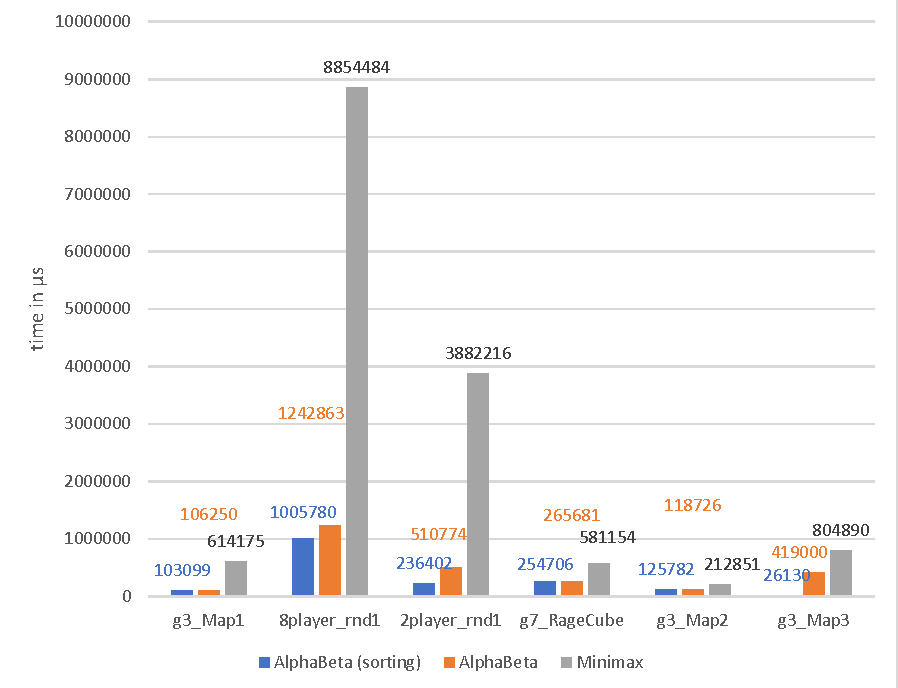
\includegraphics[scale=0.35]{Depth_2_2_avgtime}
  \end{center}
  

\end{frame}

  \begin{frame}
\frametitle{Performance}
  \begin{center}
    Durchschnittliche Zeiten pro Zug auf Tiefe 2    
    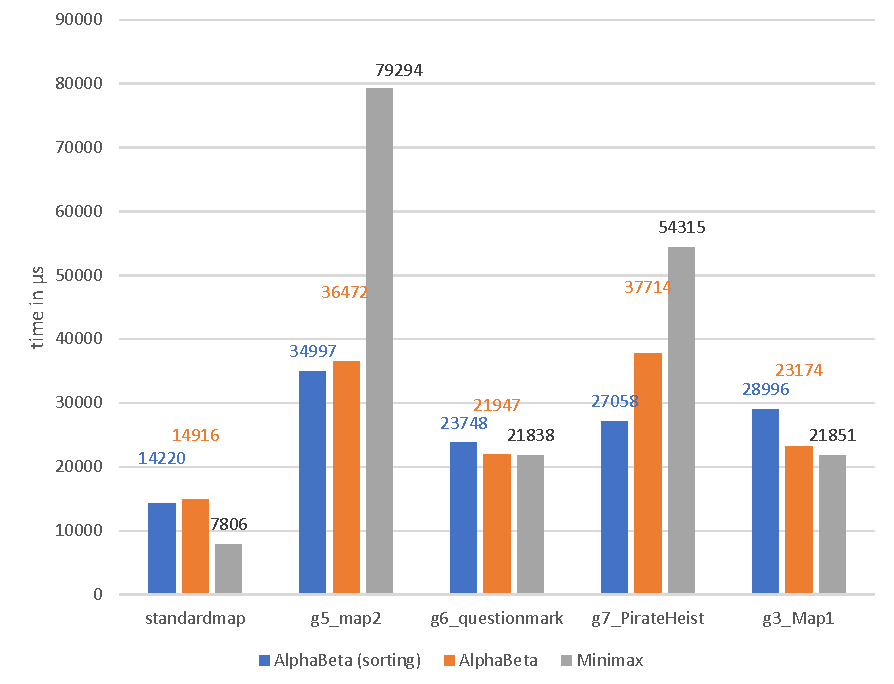
\includegraphics[scale=0.35]{Depth_2_1_avgtime}
  \end{center}
  \end{frame}

\begin{frame}
\frametitle{Performance}
  \begin{center} 
    \includegraphics[scale=0.8]{14-06_12-30-49}
  \end{center}
  
\end{frame}

%------------------------------------------------
\section{Task 3}
%------------------------------------------------

\begin{frame}
\centering
\frametitle{Iterative Deepening - Klassendiagramm}
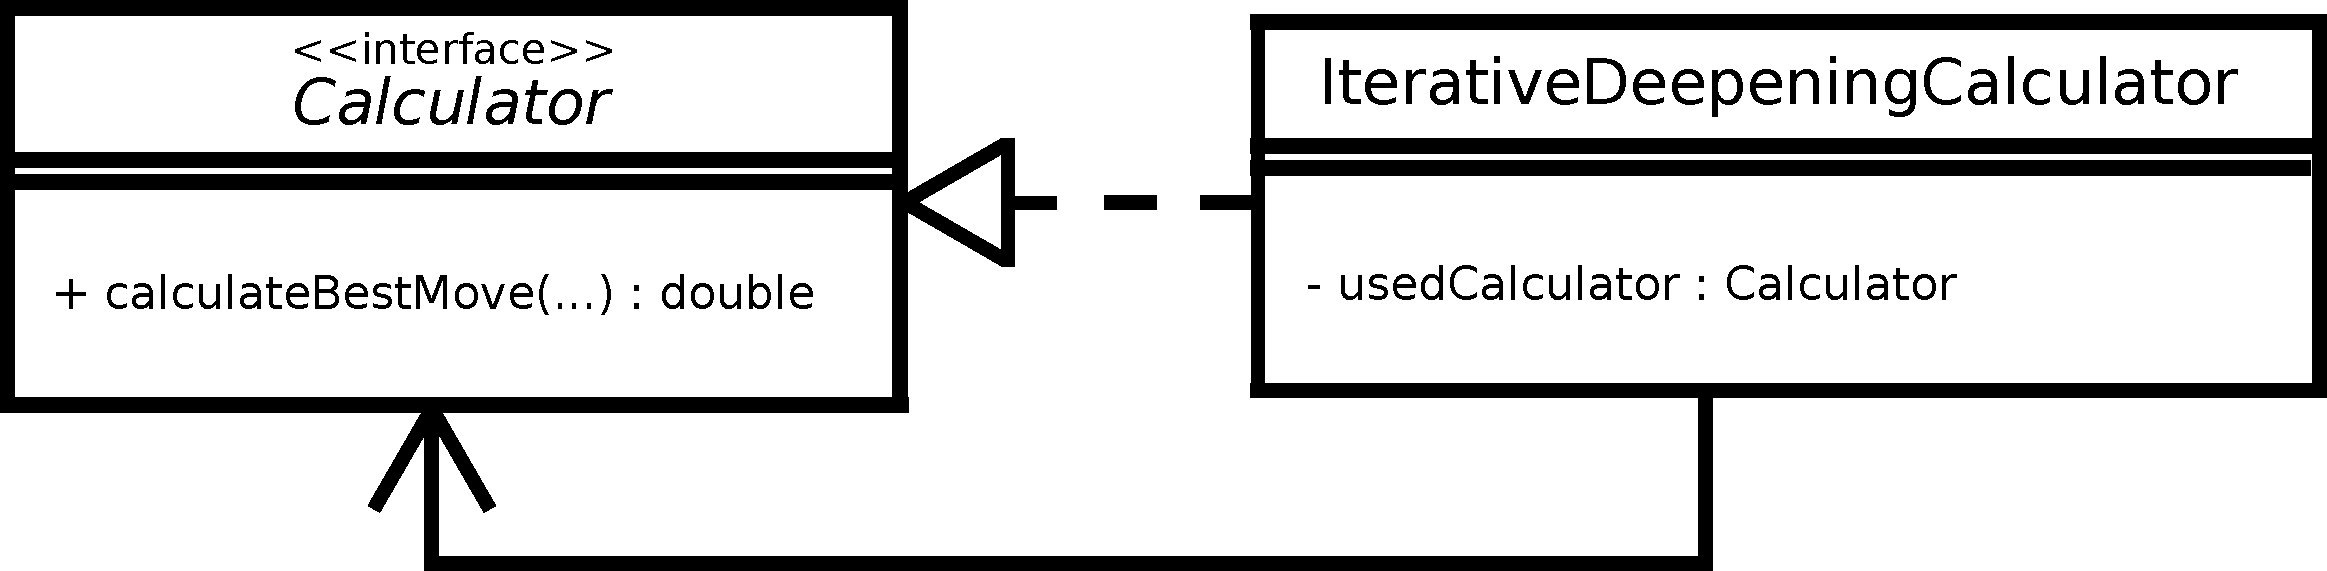
\includegraphics[scale=0.25]{deepener-classdiagram}
\end{frame}

\begin{frame}
\centering
\frametitle{Iterative Deepening - Programmfluss}
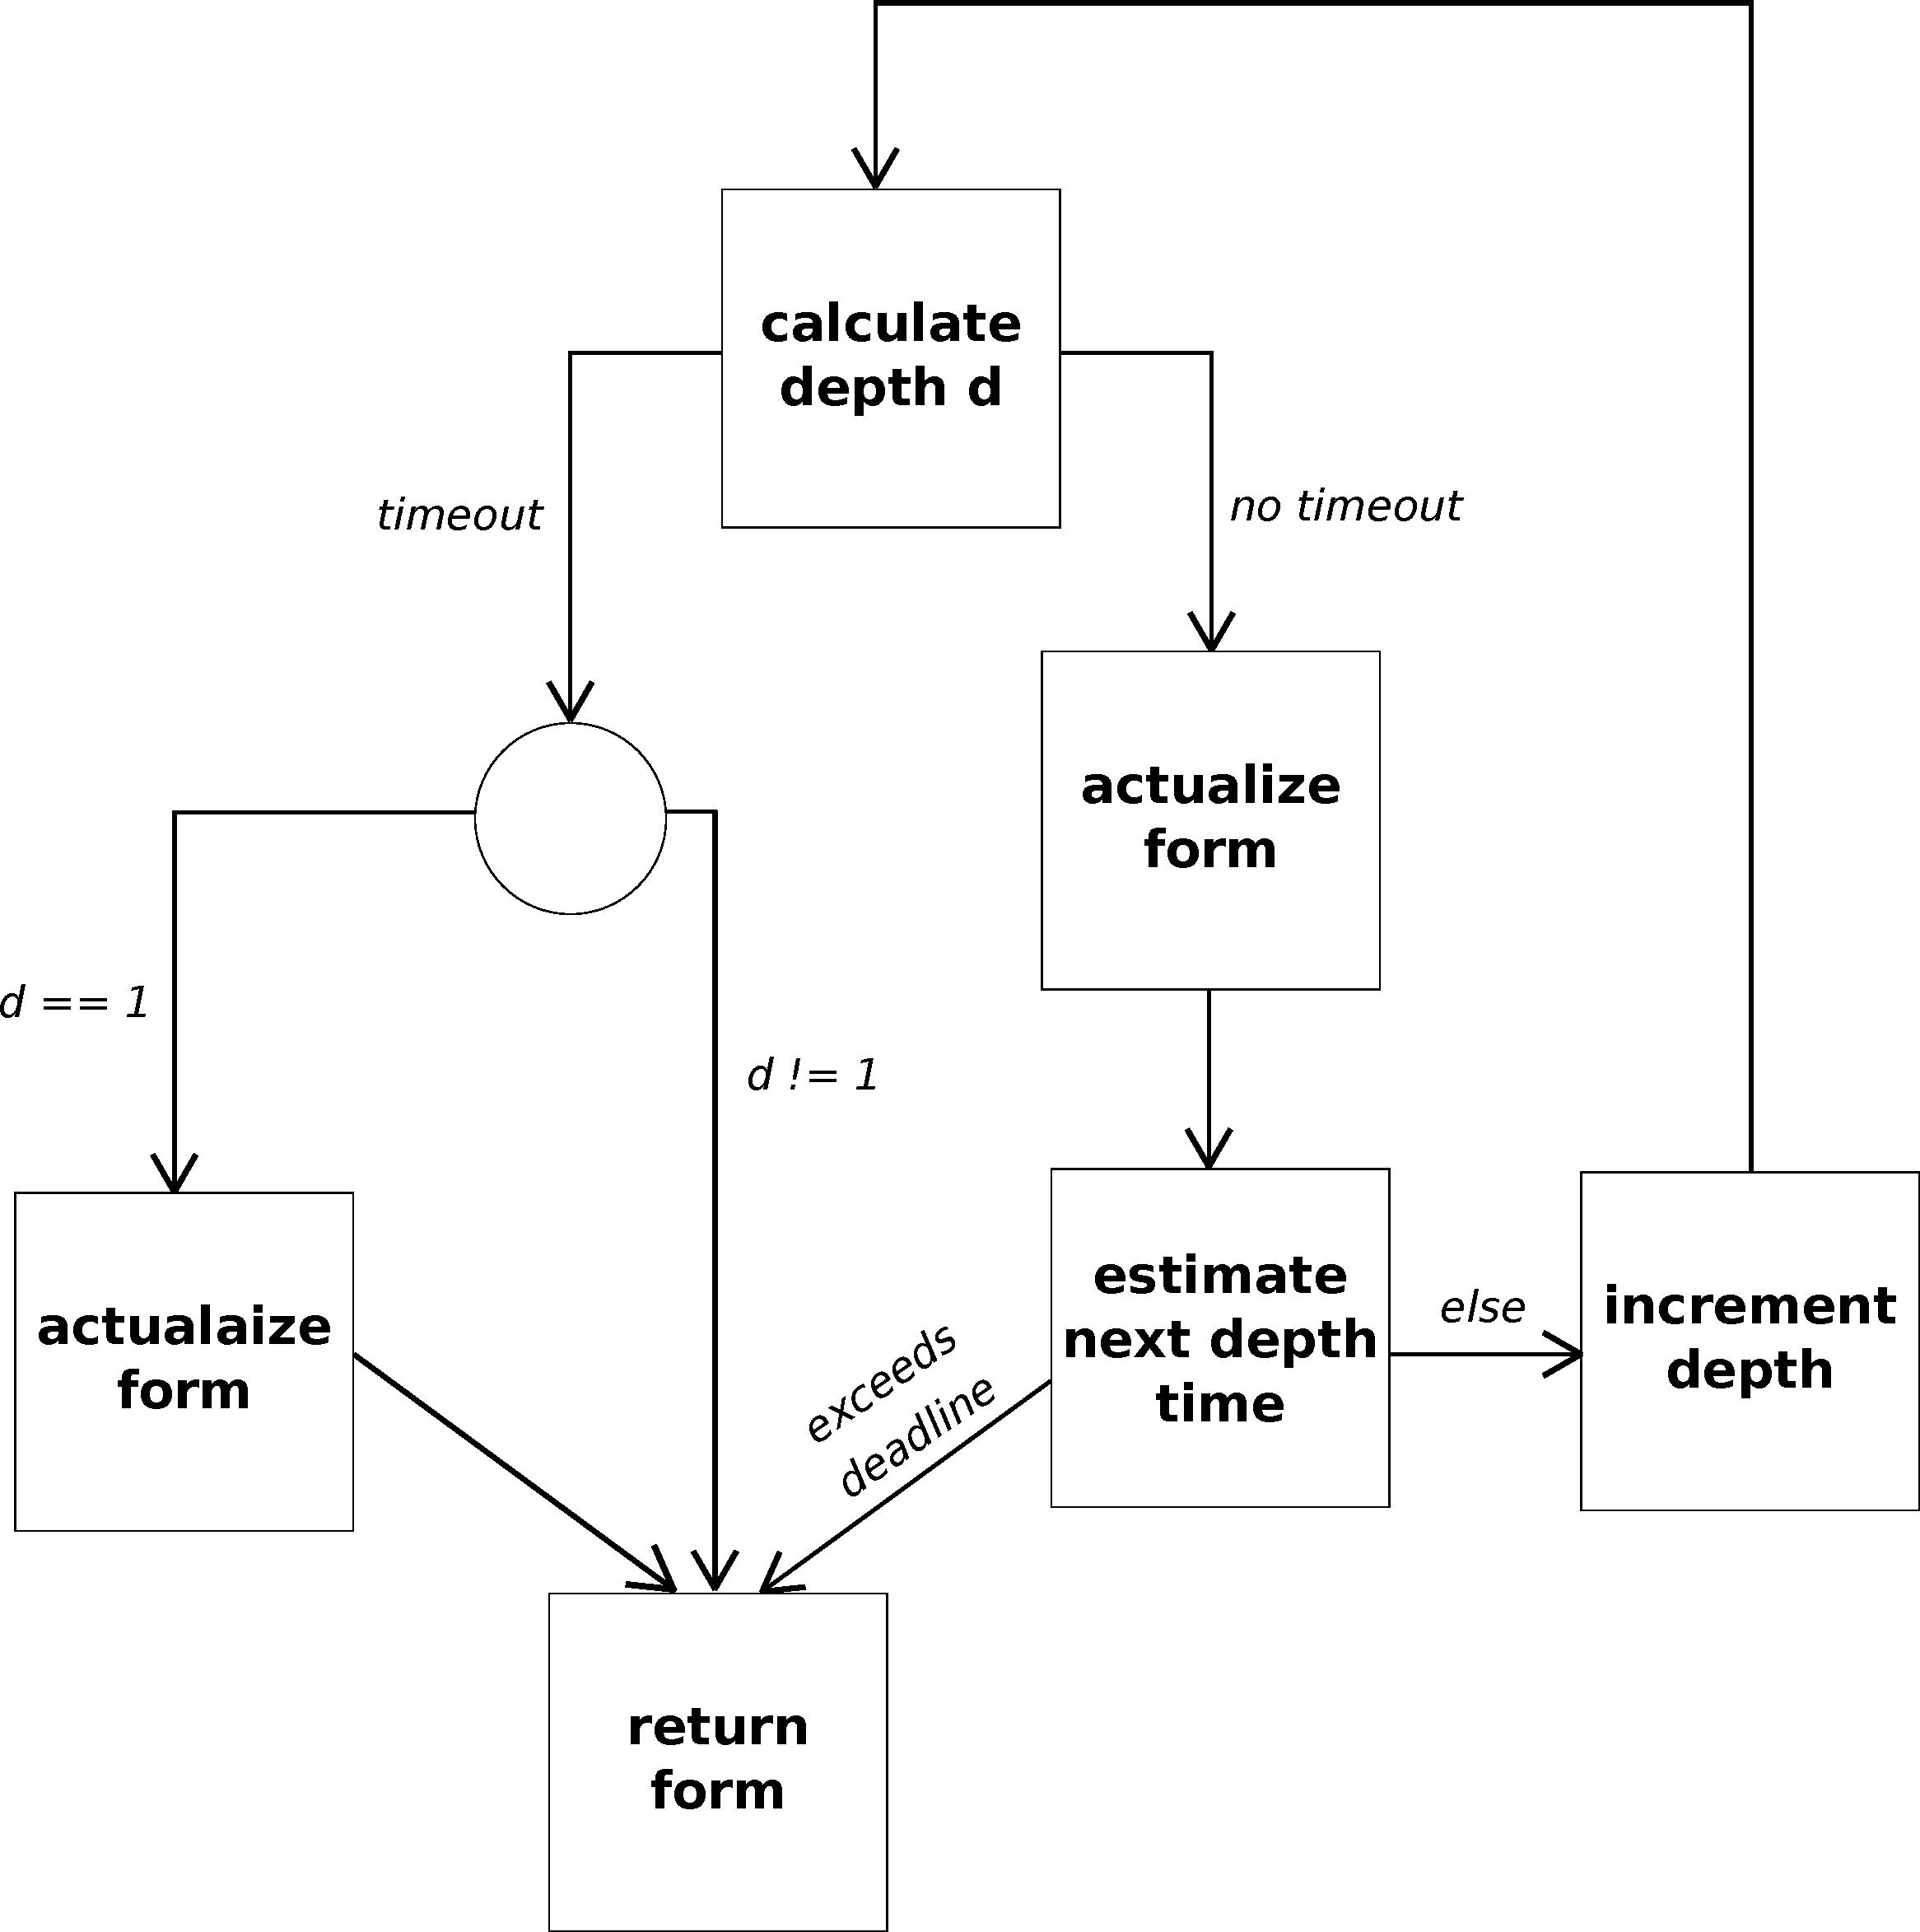
\includegraphics[scale=0.17]{deepener-flow-chart}
\end{frame}

\end{document} 